\chapter{Sahara Overview} 

\section{History}
{\em A discussion of the prevous remote sharing software, why we changed and why we chose to do it this way}

\section{What is Sahara?}
{\em A "`theory of operation"' - what Sahara is, how to develop etc}


\section{Components}
Sahara is a collection of software packages that allows a remotely control lab to be built using computer controlled equipment. This allows a large number of remote users to equitably access a limited number of rigs. It is comprised of the following modules:\\
\begin{itemize}
	\item {\bf Web Interface} through which users are authenticated and where these users can select the rigs they wish to use.  This is also the interface for administrators to manage their rigs and can provide a rig specific control interface (depending on the rig control implementation).
	\item {\bf Scheduling server} which is responsible for queuing and assigning access to rigs. It queues rigs based on a specific rig identifier: a specific rig's name, a rig's type (so that multiples of the same equipment can be treated as a group) or {\em capabilities} (a tagging system to allow identification based on behavioural or configuration identifiers).  The scheduling server also provides a registration interface to allow rigs to register themselves and declare their readiness to have users assigned to them. Determining this "`readiness"' is the domain of the Rig Client and will be described in this document in terms of the Rig Client out-of-session testing interface).
	\item {\bf The Rig Client} is the intermediary between the Scheduling server and the physical rig.  The Rig Client is explained in detail in this document.
\end{itemize}

\begin{figure}[tp]
	\centering
		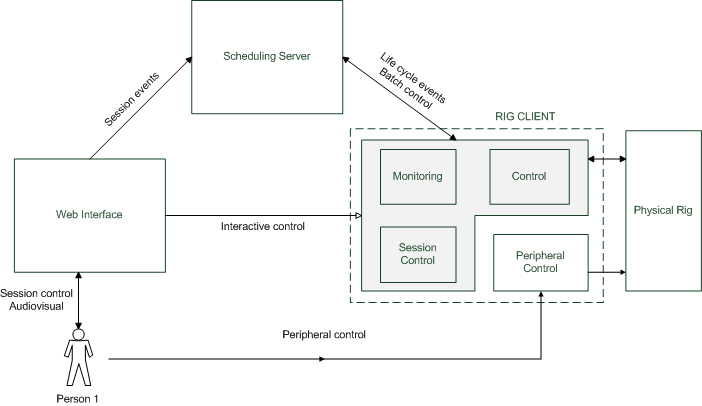
\includegraphics[scale=0.65]{Overview/SaharaSimple.png}
	\caption{Sahara architecture overview}
	\label{fig:SaharaSimple}
\end{figure}


\section{Rig Client}
The Rig Client (RC) is a software component that provides a software abstraction of a rig.  It is the intermediary between a component that decides whom may have access to the rigs (the scheduling server) and its physical hardware (the rig itself) which provides:
\begin{itemize}
	\item Session control - the mechanism of allowing externally determined users, master access to its rig (a mandatory function).  The time between granting access to the master user and revoking access from a master user is termed a �session�.
	\item Rig monitoring � testing of rig devices to ensure rig integrity (a mandatory function)
	\item Rig control - access to rig devices including control from uploaded instructions and/or direct control (an optional function). Direct control is named �primitive� control because it instructs rig devices in terms of low level operations (for example, voltages, degrees or bit register values).
\end{itemize}

The main operations of the Rig Client are to:
\begin{itemize}
 	\item allow and revoke access to a rig from master and slave users (session control);
	\item provide notification to the rig user(s) of an externally provided notification message;
	\item allow testing of a rig to determine its status as available and usable.
	\item provide rig specific information to a user, provided the user has been assigned access;
	\item provide rig control from an uploaded instruction file, provided the user has been assigned master or active slave access;
	\item provide the ability to do synchronous rig control, provided the user has been assigned master access or sufficient slave access.
\end{itemize}

\section{Web Interface}
The Web Interface is the user interface for Sahara. 

The WI has been designed to allow each institution to customise it as required.  It provides for the ability for each deployment to override certain pages and features with institution specific content. Existing default content is used if no overrides are provided. 

The mandatory development parts are the authentication of the user and the rig specific control interfaces. 
 
In Sahara 2.0 the following functionality and features are included in the WI component of Sahara:
\begin{itemize}
	\item Rig Type Page � this page is rig specific.  There are 'widgets', termed 'elements', provided to include common function components onto the rig type page (for example, an applet to launch seamless remote desktop applications), but this should be designed and implemented according to the requirements of the rig type. 
	\item Customisable common header � default Sahara headers and footers are supplied with the ability to customise these to the institution graphics.
Feedback form � ability to send feedback, or fault information on Sahara. 
 \item Contextual help dialogs � rendered place holders where information about specific pages may be provided.
	\item Login page � where users supply their login user name and password.  This function can be implemented to interface to the institution identity providers and/or �local� user authorisation can be implemented. A pluggable authentication system is provided to chain multiple authentication sources together, with associated pre-access user setup.
	\item Rig Selection Page � page displaying all the rig types and specific rigs that a user has permission to queue for.  It indicates which permissions are currently valid, which permissions have a lock associated with them and which are free to be queued for.
	\item Laboratory Rigs page � page for information on the rigs available. The default Sahara page contains images of the University of Technology, Sydney Remote Laboratory rigs.
	\item Demonstrations page � still under development, this page will allow unauthenticated access to the rigs to be used for demonstrations with appropriate configuration to set the conditions of demonstration access.
	\item News page � this page by default contains news on what has been happening with Sahara and Labshare.  It can be used for site specific information.
	\item FAQ page � this page by default has frequently asked questions about remote laboratories.  This page can be used to provide site information in a question, answer format.
	\item Contact Us page � this page by default has the contact details for Sahara Technical Development team.  It should contain details of local support contacts.
	\item Administration and reporting functionality � under development.  
\end{itemize}

\section{Scheduling Server}
{\em Similar decription of scheduling server, why it must not be modified etc}
